
%!TEX root = document.tex

%%%%%%%%%%%%%%%%%%%%%%%%%%%%%%%%%%%%%%%%%%%%%%%%%%%%%%%%%%%%%%%%%%%%%%%%%%%
\begin{table}
\centering
{\footnotesize
    \begin{tabular}{| >{\small}l | >{\small}r | }
        \hline
        \textbf{ Modality ($X$)} & $H(Y|X=true)$ \\
        \hline
        { video } & 0.850 \\
        \hline
        { link } & 0.915 \\
        \hline
        { post } & 0.918 \\
        \hline
        { photo } & 0.926 \\
        \hline
\multicolumn{2}{c}{}\\
        \hline
        \textbf{Action Type ($X$)}  & $H(Y|X=true)$ \\
        \hline
        { tags }  &  0.920 \\
        \hline
        { comments }  &  0.921 \\
        \hline
        { likes }  &  0.924 \\
        \hline
\multicolumn{2}{c}{}\\
        \hline
        \textbf{ Direction ($X$) } & $H(Y|X=true)$ \\
        \hline
        { outgoing }  &  0.928 \\
        \hline
        { incoming }  &  0.935 \\
        \hline
	\end{tabular}}
	\caption{Conditional entropy of various interactions (lower conditional
	entropies are more informative).}
	\label{table:ce_interaction}
	\vspace{-2mm}
\end{table}
%%%%%%%%%%%%%%%%%%%%%%%%%%%%%%%%%%%%%%%%%%%%%%%%%%%%%%%%%%%%%%%%%%%%%%%%%%%
%   
%%%%%%%%%%%%%%%%%%%%%%%%%%%%%%%%%%%%%%%%%%%%%%%%%%%%%%%%%%%%%%%%%%%%%%%%%%%
% %\begin{table*}
% %   \begin{tabular}{| >{\small}l | >{\small}r |}
%         \hline
%         \textbf{Modality-Direction} ($X$) & $H(Y|X=true)$ \\
%         \hline
%         tags-outgoing & 0.885 \\
%         likes-outgoing & 0.885 \\
%         tags-incoming & 0.900 \\
%         likes-incoming & 0.902 \\
%         comments-outgoing & 0.908 \\
%         comments-incoming & 0.912 \\
%         \hline
% %   \end{tabular}
% \multicolumn{2}{c}{}\\
% %   \begin{tabular}{| >{\small}l | >{\small}r |}
%                 \hline  
%         \textbf{Action-Direction} ($X$) & $H(Y|X=true)$ \\
%         \hline
%         photo-outgoing & 0.857 \\
%         video-outgoing & 0.863 \\
%         link-outgoing & 0.895 \\
%         link-incoming & 0.896 \\
%         post-incoming & 0.902 \\
%         post-outgoing & 0.906 \\
%         video-incoming & 0.915 \\
%         photo-incoming & 0.921 \\
%         \hline
                
%     \end{tabular}}
% \end{table}
%%%%%%%%%%%%%%%%%%%%%%%%%%%%%%%%%%%%%%%%%%%%%%%%%%%%%%%%%%%%%%%%%%%%%%%%%%%

%%%%%%%%%%%%%%%%%%%%%%%%%%%%%%%%%%%%%%%%%%%%%%%%%%%%%%%%%%%%%%%%%%%%%%%%%%%
%\begin{figure*}[tbp!]
%\centering
%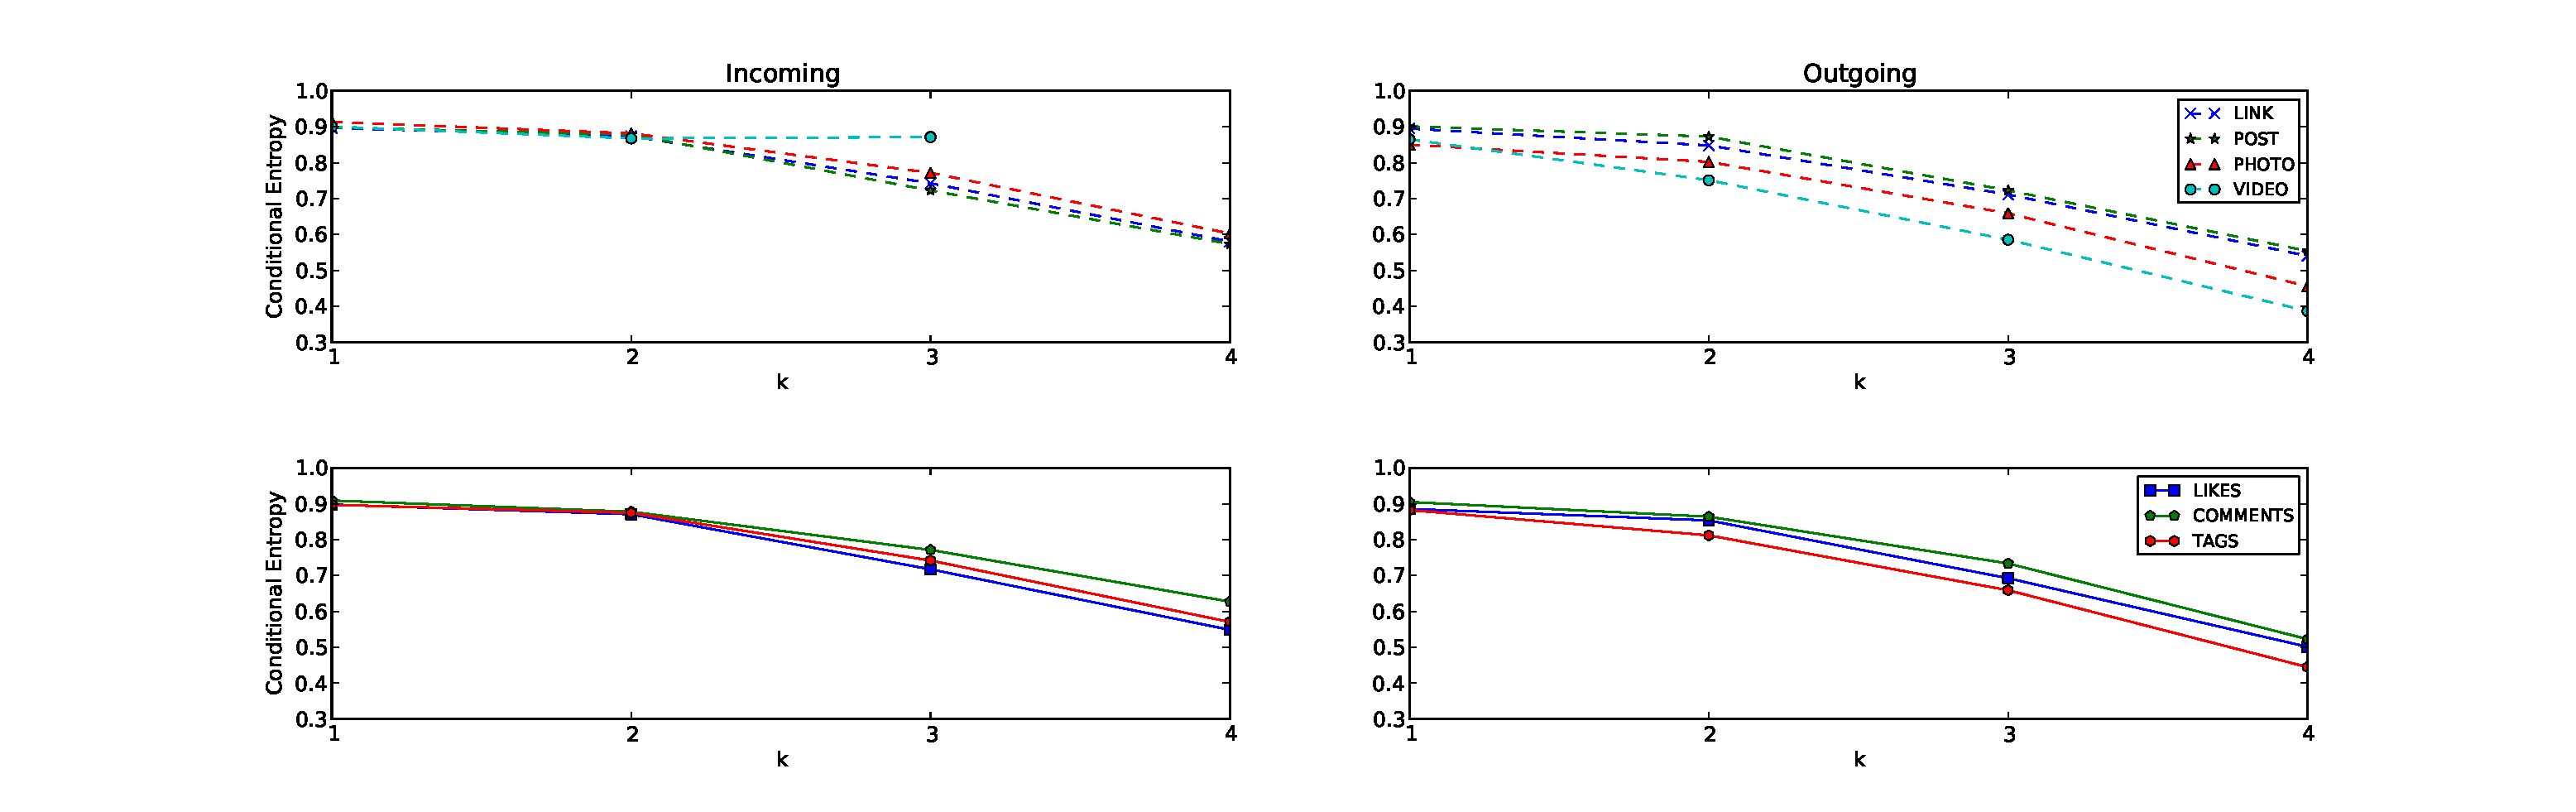
\includegraphics[height=50mm,width=160mm]{data/plots/vsk/ModalityActionsvsKFriends.eps}
%\caption{Conditional Entropy  of modalities/activities for incoming/outgoing interactions vs item liked by at least k friends}
%\label{Fig2} 
%\end{figure*}
%%%%%%%%%%%%%%%%%%%%%%%%%%%%%%%%%%%%%%%%%%%%%%%%%%%%%%%%%%%%%%%%%%%%%%%%%%%
In this section we analyze the informativeness of Interaction SAGs,
namely user interactions according to their modality, type, and direction, 
as described in Section~\ref{sec:methodology}. Similarly, we analyze the relationship between
informativeness of Activity SAGs and its size.

%namely those SAGs that are built w.r.t. a user $u$'s interactions.
A general method for measuring the amount of information that a 
feature $X$ provides w.r.t. predicting another variable $Y$ (in this
case likes or dislikes) is to calculate its conditional entropy:
\begin{align*}
H(Y&|X=True)\\
& = -\sum_{y\in{(\like,\dislike)}} p(y|X=true) \ln( p(y|X=true))
\end{align*}

In general, a lower conditional entropy indicates a more informative
feature. Here we use entropy conditioned on sparse features $X=True$ 
instead of just $H(Y~|~X)$ or mutual information $I(Y; X)$, as we found 
that the alternatives are highly correlated with (or dominated by) the number of 
occurrences of the feature (or $P(X=True)$), and give trivial results. 

%As defined in Sec~\ref{sec:methodology}, we have three distinctions for user
%interactions: modality, action, and directionality. 
Table~\ref{table:ce_interaction} shows the conditional entropy for Interactions based on modality, action and direction. Here we observe,
\begin{itemize}
\item Interaction on {\em videos} seem to have a stronger preferential affinity 
than other modalities such as links, posts and photos.  This could be
  due to the fact that video viewing is time-consuming and users
  inherently only watch the videos of those whose preferences they
  often share.
\item Tagging has a slightly lower conditional entropy than
  commenting and liking, likely because the majority of tags contains 
  person name(s) on Facebook, indicating a direct social interaction. 
  % indicating that tagging.
\item A user is more likely to share preferences with someone who she
  initiates the interaction with (outgoing) vs. with someone who
  initiates the interaction with her (incoming).  
\end{itemize}

% First we analyze various interactions individually and jointly to understand what
% interactions define SAGs with a high social affinity for a user $u$'s
% preferences.  To this end, we make a few observations from the
% conditional entropy analysis of Table~\ref{table:ce_interaction}:
% \begin{itemize}
% \item Interaction on {\em videos} seem to have a stronger preferential affinity 
% than other modalities such as links, posts and photos.  This could be
%   due to the fact that video viewing is time-consuming and users
%   inherently only watch the videos of those whose preferences they
%   often share.
% \item Tagging has a slightly lower conditional entropy than
%   commenting and liking, likely because the majority of tags contains 
%   person name(s) on Facebook, indicating a direct social interaction. 
%   % indicating that tagging.
% \item A user is more likely to share preferences with someone who she
%   initiates the interaction with (outgoing) vs. with someone who
%   initiates the interaction with her (incoming).  As an extreme
%   instance of this, we note that while outgoing photo and video
%   interactions are most informative, it appears that incoming photo
%   and video interactions are least informative.
% \end{itemize}

% In figure \ref{Fig2} we plot conditional entropy of modality and
% action for incoming/outgoing interactions constrained to links
% liked by at least $k$ friends in the Interaction SAG.  Figure \ref{Fig2} reiterates
% many observations made above for various $k$.  In addition, we note that
% preference affinity with a SAG increases as more people in the SAG
% Note that these graphs are cumulative in $k$, different from the 
% exposure curve on exactly $k$ friends~\cite{Romero2011hashtag}. 
% Our observations on user preference on items like by a number of Facebook friends 
% suggest large cumulative number of friend interactions is more predictive 
% -- this can be translated into recommender system design. 
% Further investigation is needed to pinpoint whether or not there is 
% diminishing returns on repeated exposures~\cite{ver2011stops,Romero2011hashtag} on $k$, 
% and how this could be leveraged to design recommendation algorithms.


%We observed that 
%\begin{itemize}
%% NOTED ABOVE NOW
%  \item Some interactions are more predictive than other. For
%    eg. videos and photo interactions were found to be significantly
%    more predictive than post and link interactions. Similarly,
%    tagging action is often more predictive than commenting and
%    liking.
%  \item As noted by previous work~\cite{saez2011high}, we observe that
%    outgoing interactions are more predictive than incoming
%    interactions. Furthermore, the differentiation between
%    predictiveness modalities and actions is more pronounced in
%    outgoing interactions than in incoming interactions.
%  \item 

%This exhibits repeated exposure properties of epidemic
%models for social networks~\cite{Golub2010selectionbiase}.
%\end{itemize}


%!TEX root = document.tex

% Note: activity SAGs can go beyond friends.

%In this section we evaluate the correlation between the conditional
%entropy and size of groups, pages and favourites.

Fig \ref{Fig3} shows the relationship between conditional
    entropy versus the size of activity groups. 
    Here the size of a {\em group}, {\em page} and {\em favorite} 
    is the number of total users in the activity group.  
    For {\em Pages} and {\em Favorites} this is the total number of Facebook users, 
    while for {\em Groups} only the number of users in the App users' ego network 
    is visible to our app. \ref{Fig3} shows that the activity groups of 
    small size can be highly predictive whereas large groups are rarely predictive.

In Fig~\ref{Fig4} we plot the average conditional entropy of the top
    10\% of features cumulative up to the size of the activity group given on the
    x-axis; this allows us to determine the marginal contribution of
    larger groups to the average conditional entropy as larger groups
    are incrementally added in.  This graph 
    distinctly shows that the small sized groups, pages and favourites
    have low average conditional entropy that transitions sharply to a
    higher average once a size threshold has been met.From 
    Fig~\ref{Fig4} we can infer that the group sizes up to 50 and
    page/favourite sizes up to $10^{5}$ are most predictive.
    
    
    In Fig~\ref{Fig5}  we analyze the predictiveness of favourites by categories.
    We can see that contents in the ``long-tail'', i.e.,  
    having a large number of occurrences far from the most popular choices, 
    tend to have be the most predictive affinities. Examples of these include
    music, books, movies. On the contrary, generic affinities (e.g. interests) and 
    those with a smaller number of choices (e.g. sports or fav-teams) 
    tend to be less predictive. 

% %{\bf TODO: make this consistent with earlier discussion regarding persistence,
% %temporally sychronized.}

%     We also analyze predictiveness of favourites by categories in
%     Fig~\ref{Fig5}, where the favorite categories are obtained from Facebook API. 

%     %It shows that SAGs consisting of shared interests,
%     %activity, television, and books are on average most predictive, while 
%     %music, movies, favourite teams, sports and athletes are on average
%     %least predictive.  
   
%     We can see that contents in the ``long-tail'', i.e.,  
%     having a large number of occurrences far from the most popular choices, 
%     tend to have be the most predictive affinities. Examples of these include
%     music, books, movies. On the contrary, generic affinities (e.g. interests) and 
%     those with a smaller number of choices (e.g. sports or fav-teams) 
%     tend to be less predictive. 
   
%     %While favourite teams, sports and athletes may be
%     %too focused to offer much predictiveness vs. the other more diverse
%     %categories, it is interesting that movies and music favourites
%     %are not very predictive on average.  This may have to do with the fact that
%     %these are typically ephemeral favourites that may be heavily influenced
%     %by popularity as opposed to true personal preference.
% %\end{itemize}

%In Fig~\ref{Fig4} we plot the average conditional entropy of top
%    10\% features cumulative over the size of activity group. It
%    distinctly shows that the small sized group, pages and favourites
%    have low average conditional entropy. Furthermore, it explains
%    average conditional entropy decreases as size increases. From the
%    figure \ref{Fig4} we can infer that the group size upto 50 and
%    page/favourite size upto $10^{5}$ can be highly predictive.
%
%We also analyze predictiveness of favourites by categories in
%    Fig \ref{Fig5}. It shows that television, books, music and movies
%    are predictive whereas favourite teams, sports and athletes are
%    less predictive.
%\end{itemize}

% %\TODO{add a table of top 5-10 groups/pages/favs}

% \begin{table*}[tbp!]
% \centering
% \begin{tabular}{| >{\small}l | >{\small}r | >{\small}r |}
% \hline
% \textbf{Top Groups} & \textbf{Top Pages} & \textbf{Top Favourites} \\
% \hline
% %Heavy Metal - Australian Capital Territory & Avascular Necrosis & Avascular Necrosis \\
% Heavy Metal - (city name) & Avascular Necrosis & Avascular Necrosis \\
% Stephen Conroy Should Not Filter Our Internet & Assidian & Tortured \\
% Silicone Stripper & Tortured & Elysian \\
% Hardcore dancing is not moshing & Elysian & Anno Domini \\
% %Metal bands come to Canberra cause I'm sick of... & Darker Half & Hellbringer \\
% Metal bands come to (city name) cause I'm sick of... & Darker Half & Hellbringer \\
% %Canberra Rock Gigs & Johnny Roadkill & Johnny Roadkill \\
% (city name) Rock Gigs & Johnny Roadkill & Johnny Roadkill \\
% %Let's Mosh - Canberra metal radio show - 2XX 9 & Anno Domini & Darker Half \\
% Let's Mosh - (city name) metal radio show - 2XX 9 & Anno Domini & Darker Half \\
% Bring Steel Panther to Australia & Billy Madison & Bane Of Isildur \\
% %Canberra Death/Heavy Metal Appreciation & Hellbringer & Katabasis \\
% (city name)  Death/Heavy Metal Appreciation & Hellbringer & Katabasis \\
% Robert The Bruce (Band) & Metalocalypse & Aeon of Horus \\
% \hline
% \end{tabular}
% \caption{Top 10 Groups/Pages/Favourites ranked by Conditional Entropy. The city name where our institution and many Facebook users resides is anonymized.}
% \label {table:topGroupPagesFavs}
% \end{table*}



%%%%%%%%%%%%%%%%%%%%%%%%%%%%%%%%%%%%%%%%%%%%%%%%%%%%%%%%%%%%%%%%%%%%%%%%%%%
\begin{figure}[tbp!]
%\centering
\hspace{-8mm}
\begin{tabular}{ccc}
\subfloat[Fig:][]{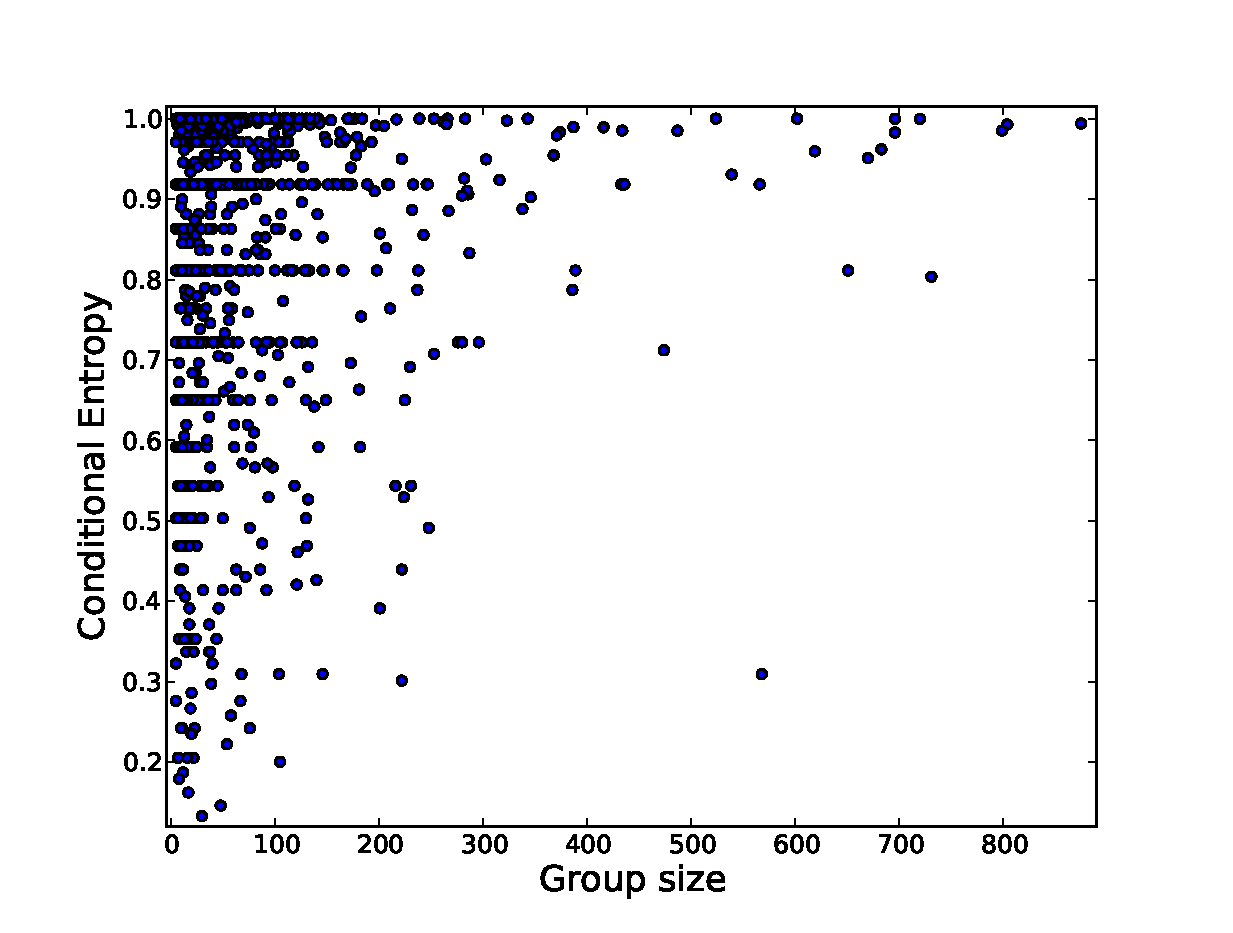
\includegraphics[width=32mm, height=30mm]{data/plots/new/CEvsGroupSize.eps}}
\subfloat[Fig:][]{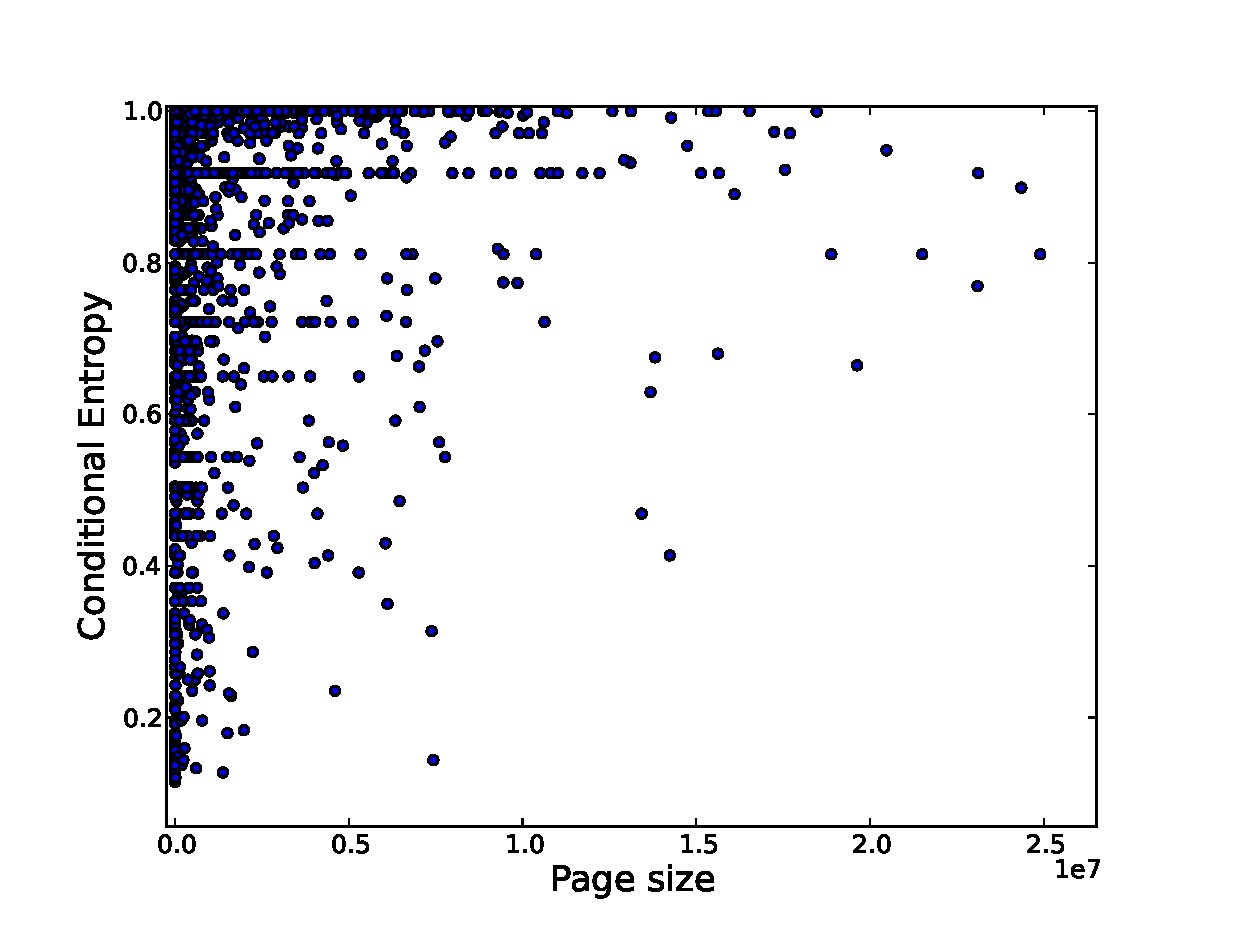
\includegraphics[width=32mm, height=30mm]{data/plots/new/CEvsPageSize.eps}}
\subfloat[Fig:][]{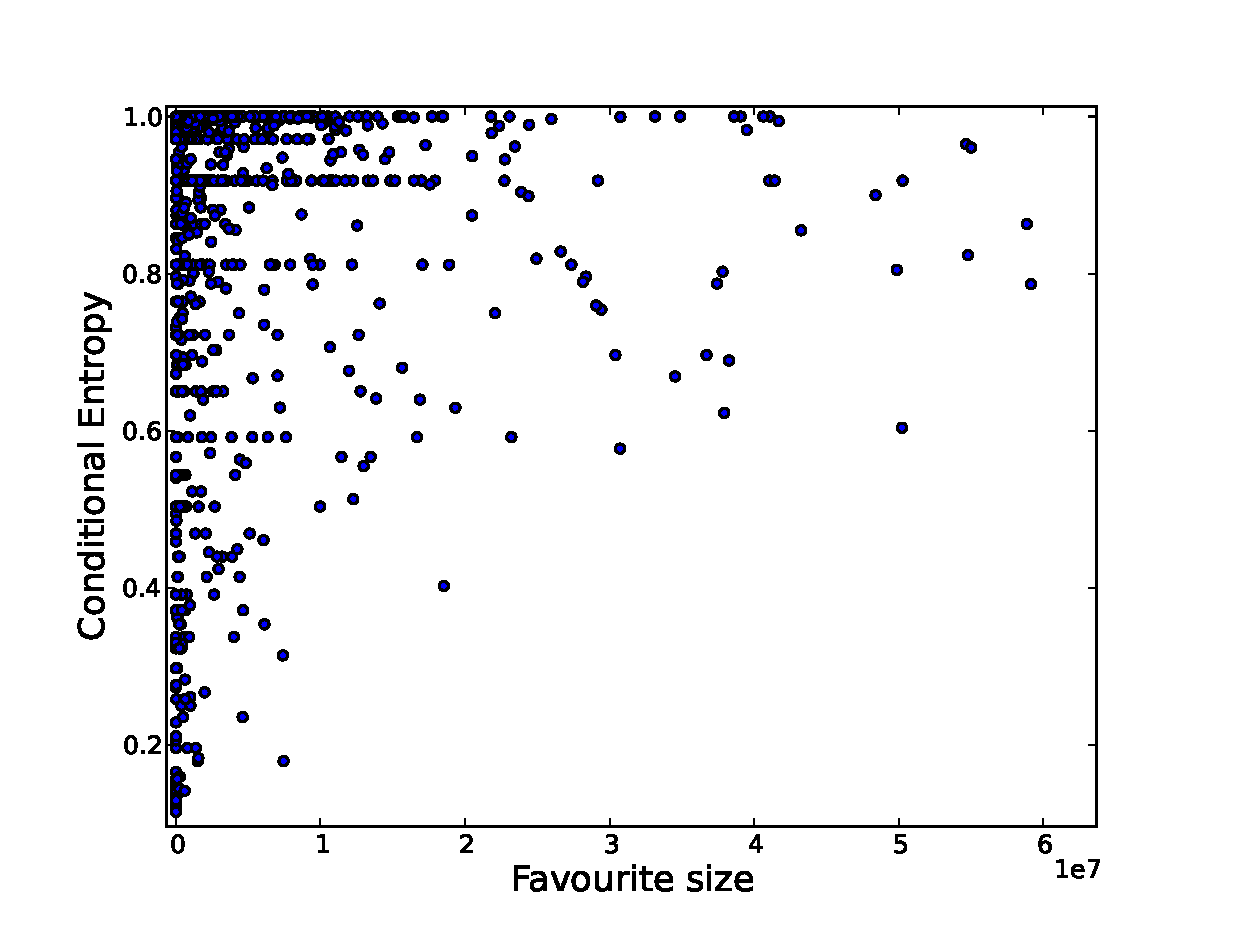
\includegraphics[width=32mm, height=30mm]{data/plots/new/CEvsFavSize.eps}}
\end{tabular}
\caption {Conditional entropy vs size }
\label{Fig3}
\end{figure}
%%%%%%%%%%%%%%%%%%%%%%%%%%%%%%%%%%%%%%%%%%%%%%%%%%%%%%%%%%%%%%%%%%%%%%%%%%%

% %%%%%%%%%%%%%%%%%%%%%%%%%%%%%%%%%%%%%%%%%%%%%%%%%%%%%%%%%%%%%%%%%%%%%%%%%%%
% \begin{figure}[tbp!]
% %\centering
% \hspace{-10mm}
% \begin{tabular}{ccc}
% \begin{tabular}{ccc}
% \subfloat[Fig:][]{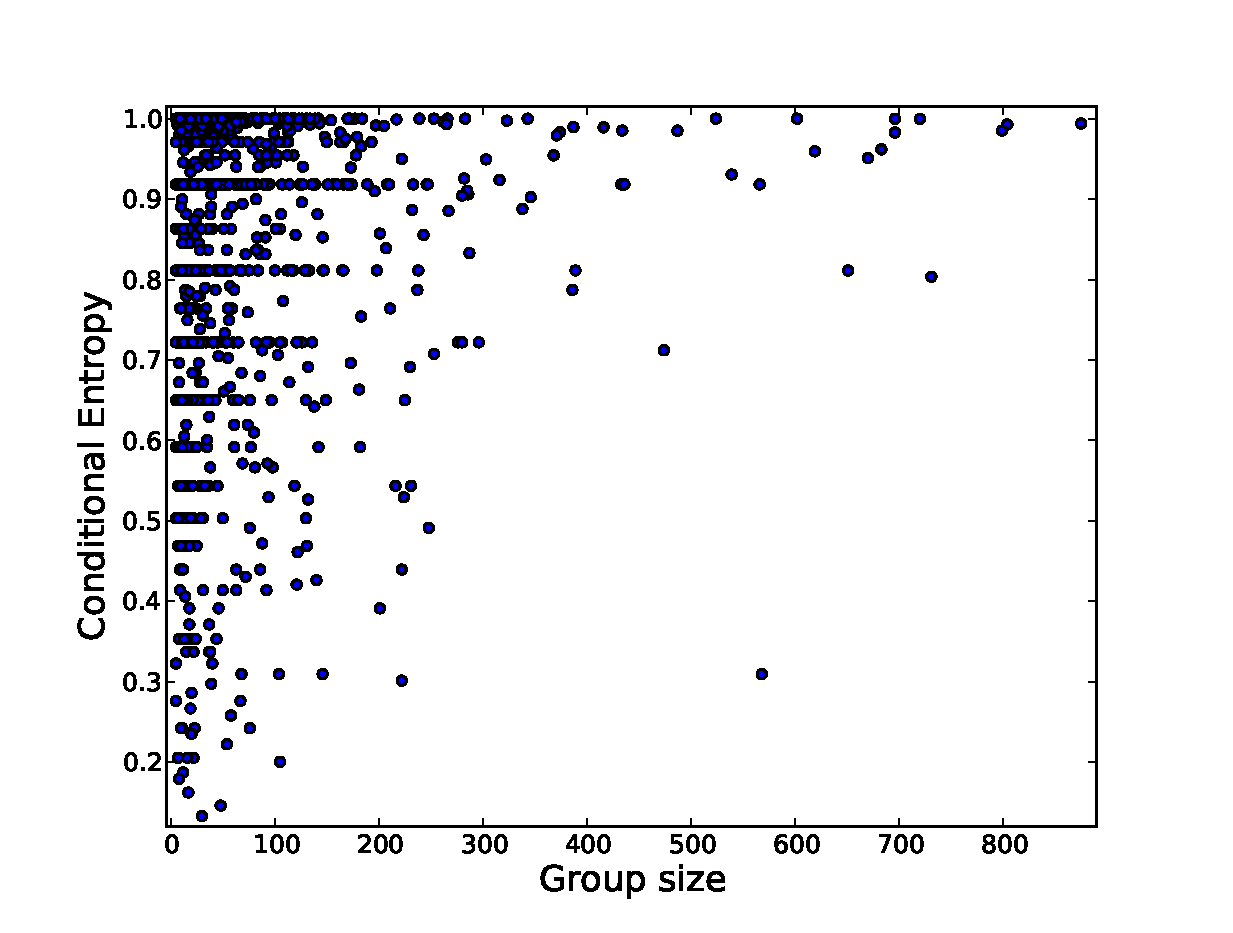
\includegraphics[width=32mm, height=30mm]{data/plots/new/CEvsGroupSize.eps}}
% \subfloat[Fig:][]{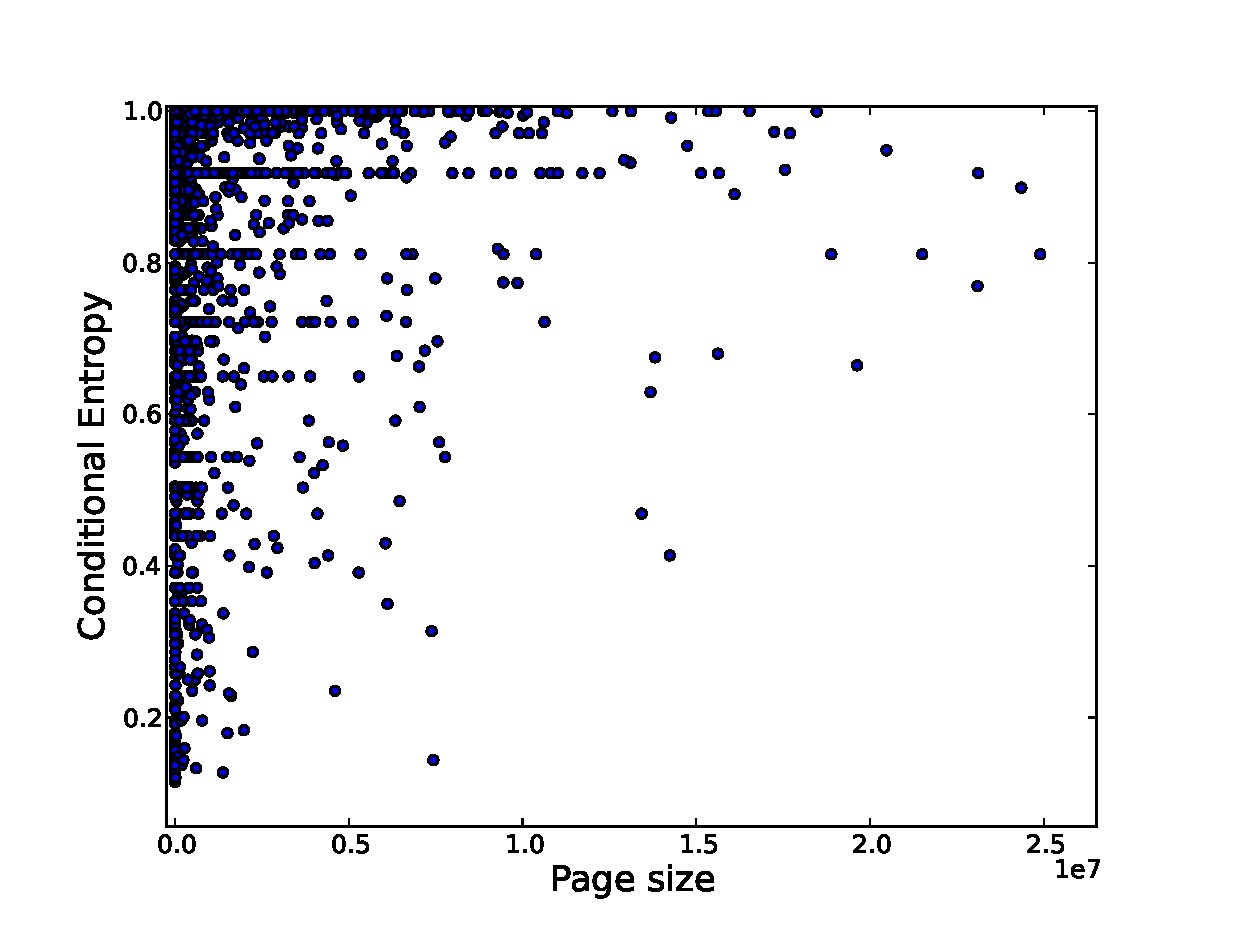
\includegraphics[width=32mm, height=30mm]{data/plots/new/CEvsPageSize.eps}}
% \subfloat[Fig:][]{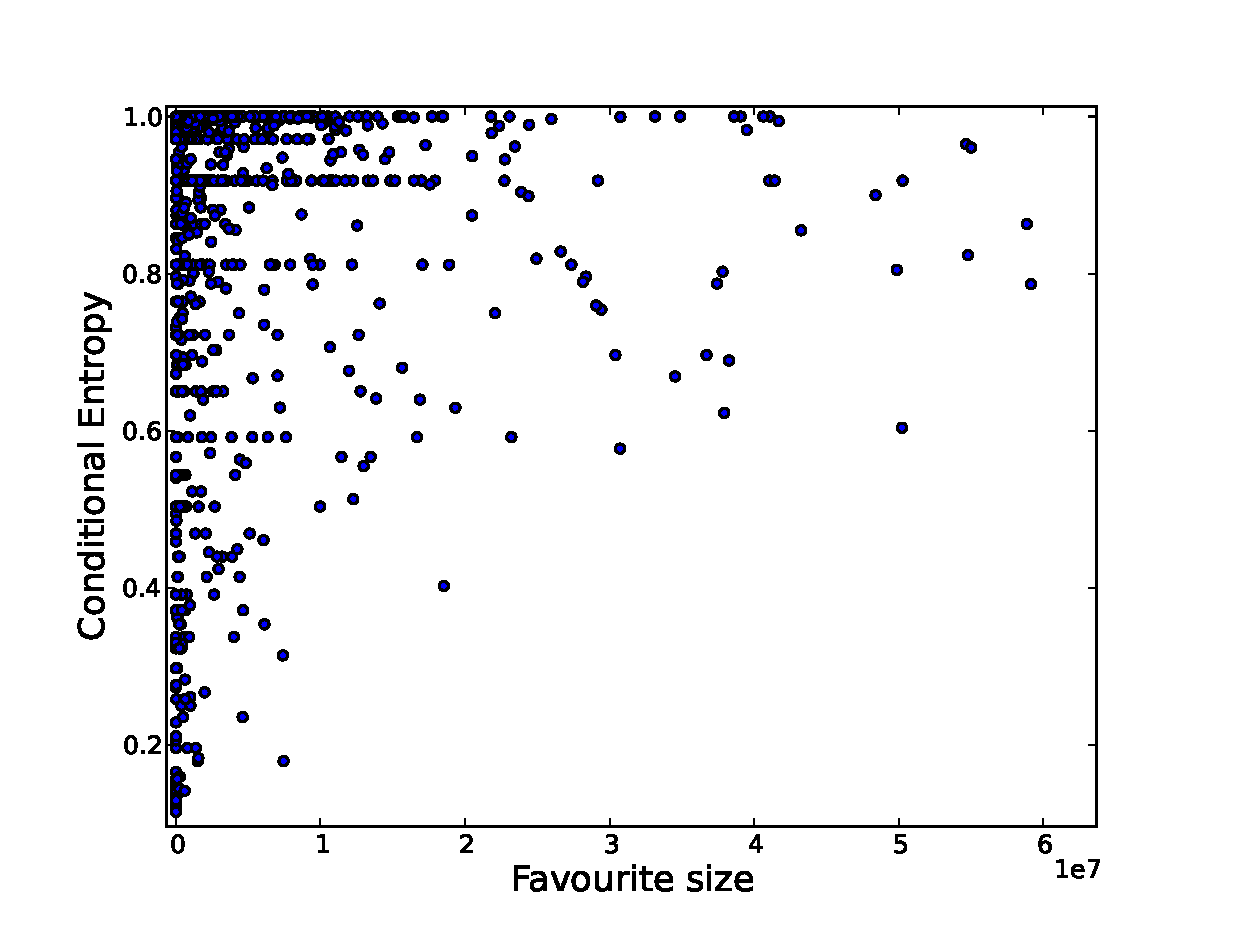
\includegraphics[width=32mm, height=30mm]{data/plots/new/CEvsFavSize.eps}} \\
% \subfloat[Fig:][]{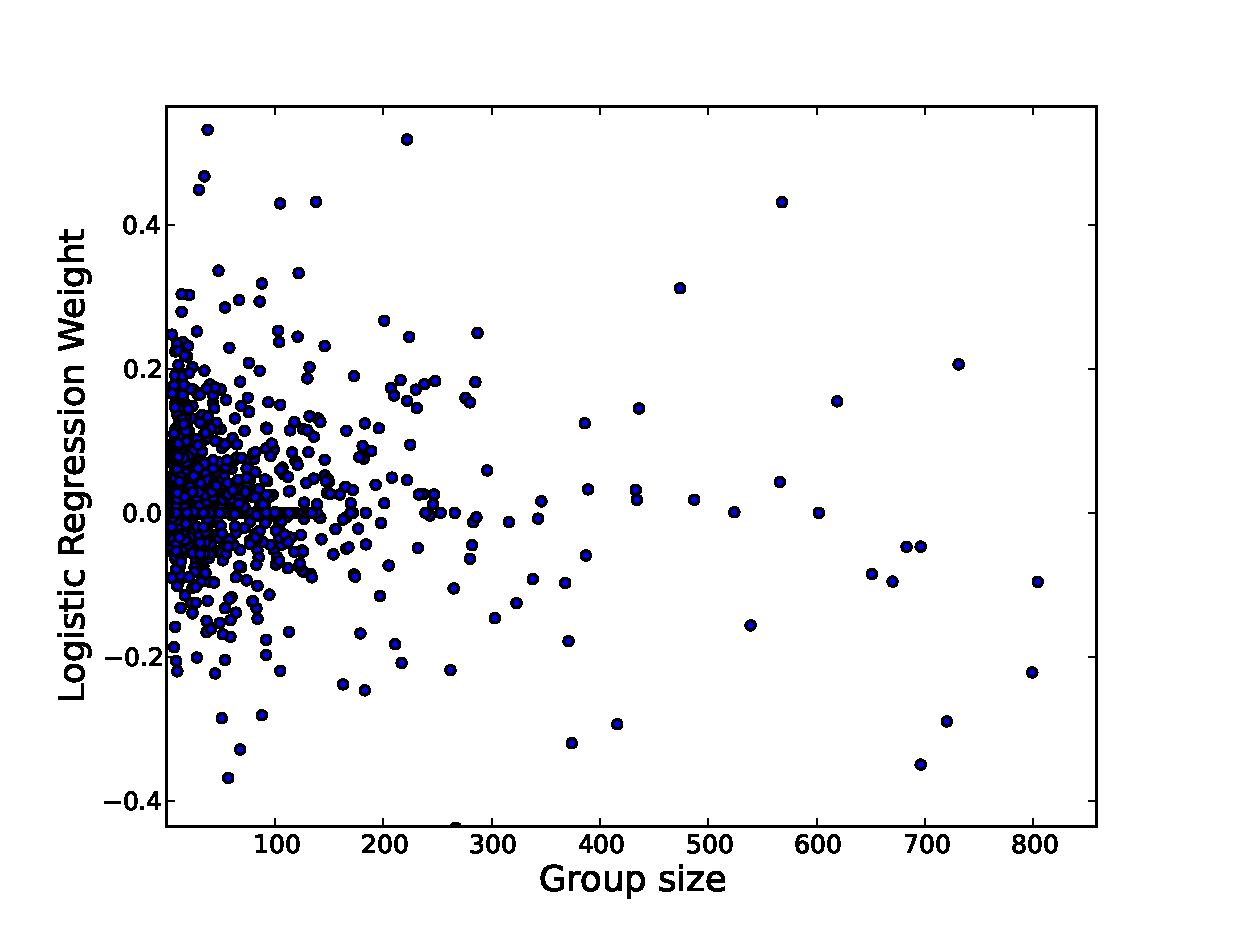
\includegraphics[width=32mm, height=30mm]{data/plots/new/LRweightvsGroupSize.eps}}
% \subfloat[Fig:][]{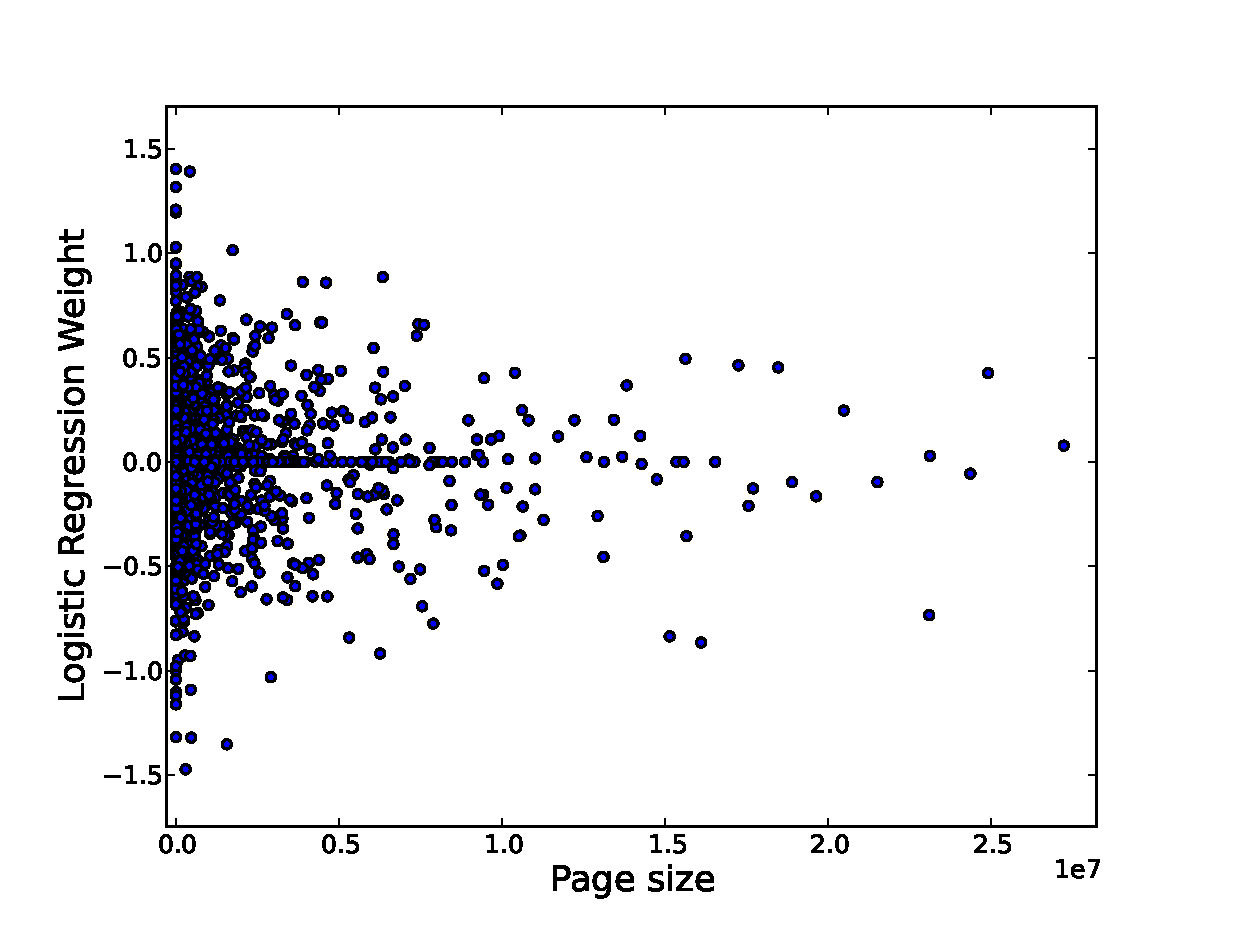
\includegraphics[width=32mm, height=30mm]{data/plots/new/LRweightvsPageSize.eps}}
% \subfloat[Fig:][]{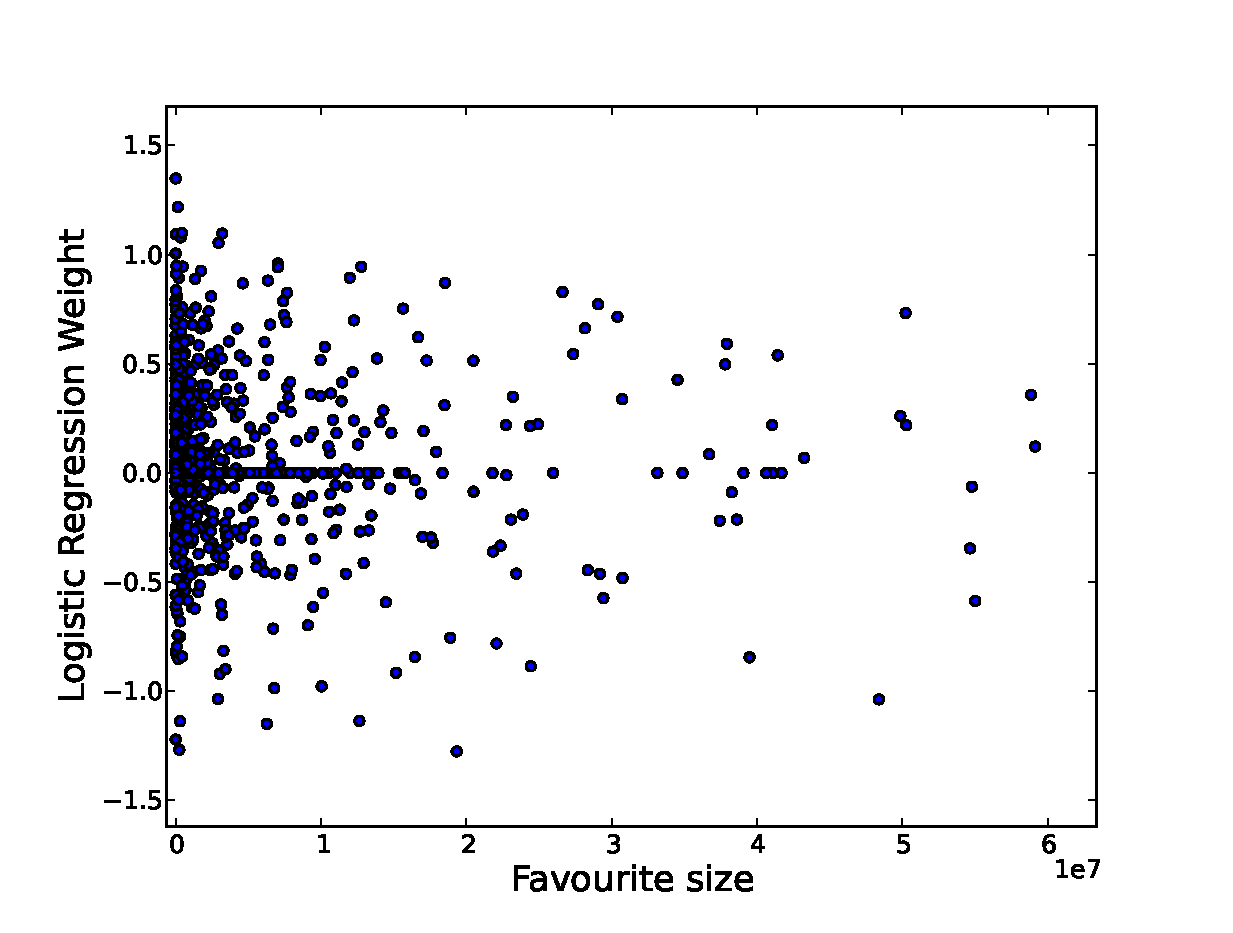
\includegraphics[width=32mm, height=30mm]{data/plots/new/LRweightvsFavSize.eps}} \\
% \end{tabular}
% \end{tabular}
% \caption {Conditional entropy vs size (a-c); logistic regression feature weights vs size (d-f) }
% \label{Fig3}
% \end{figure}
% %%%%%%%%%%%%%%%%%%%%%%%%%%%%%%%%%%%%%%%%%%%%%%%%%%%%%%%%%%%%%%%%%%%%%%%%%%%

%%%%%%%%%%%%%%%%%%%%%%%%%%%%%%%%%%%%%%%%%%%%%%%%%%%%%%%%%%%%%%%%%%%%%%%%%%%
\begin{figure*}[tbp!]
\centering
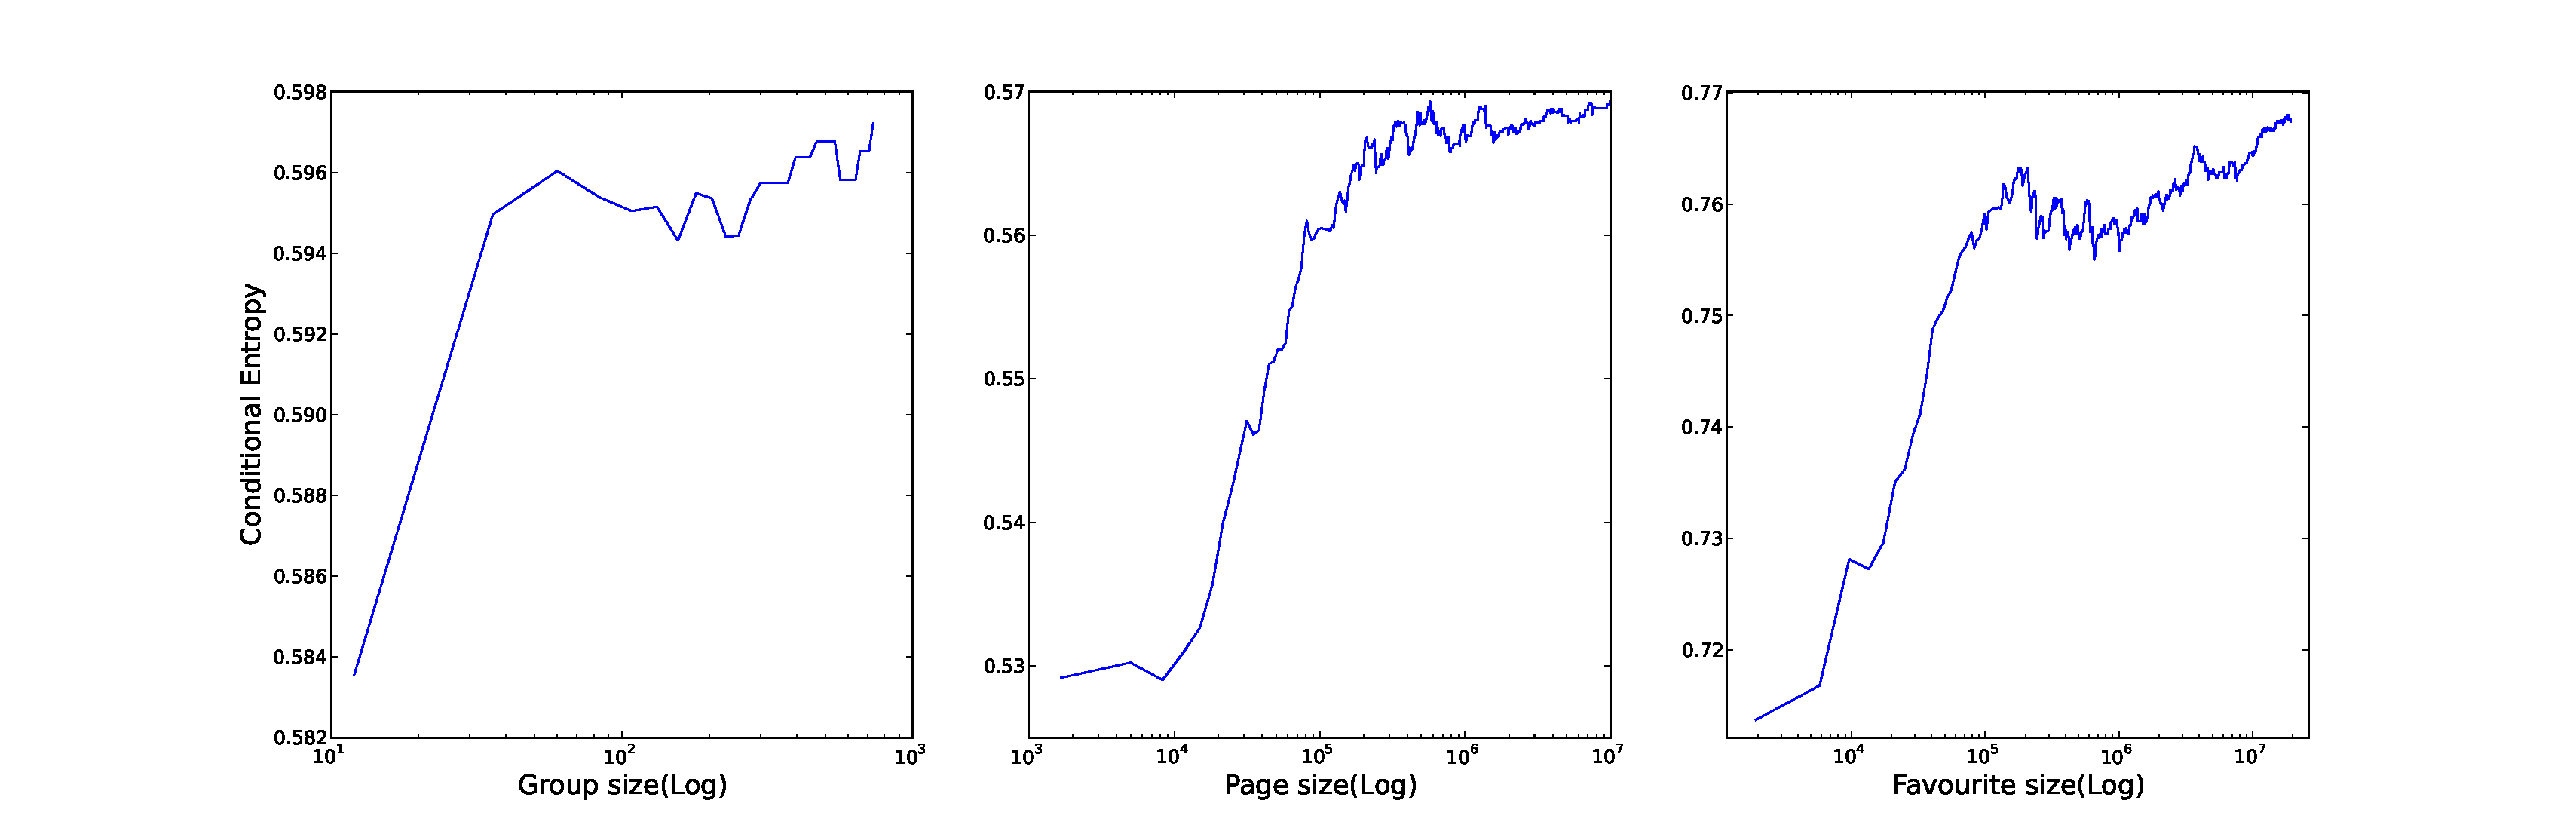
\includegraphics[width=160mm,height=40mm]{data/plots/cumulativeEntropy/cumulative.eps}
\caption{Average conditional entropy of top 10\% groups, pages and favourites features cumulative over the size }
\label{Fig4}
\end{figure*}
%%%%%%%%%%%%%%%%%%%%%%%%%%%%%%%%%%%%%%%%%%%%%%%%%%%%%%%%%%%%%%%%%%%%%%%%%%%

%%%%%%%%%%%%%%%%%%%%%%%%%%%%%%%%%%%%%%%%%%%%%%%%%%%%%%%%%%%%%%%%%%%%%%%%%%%
\begin{figure*}[tbp!]
\centering
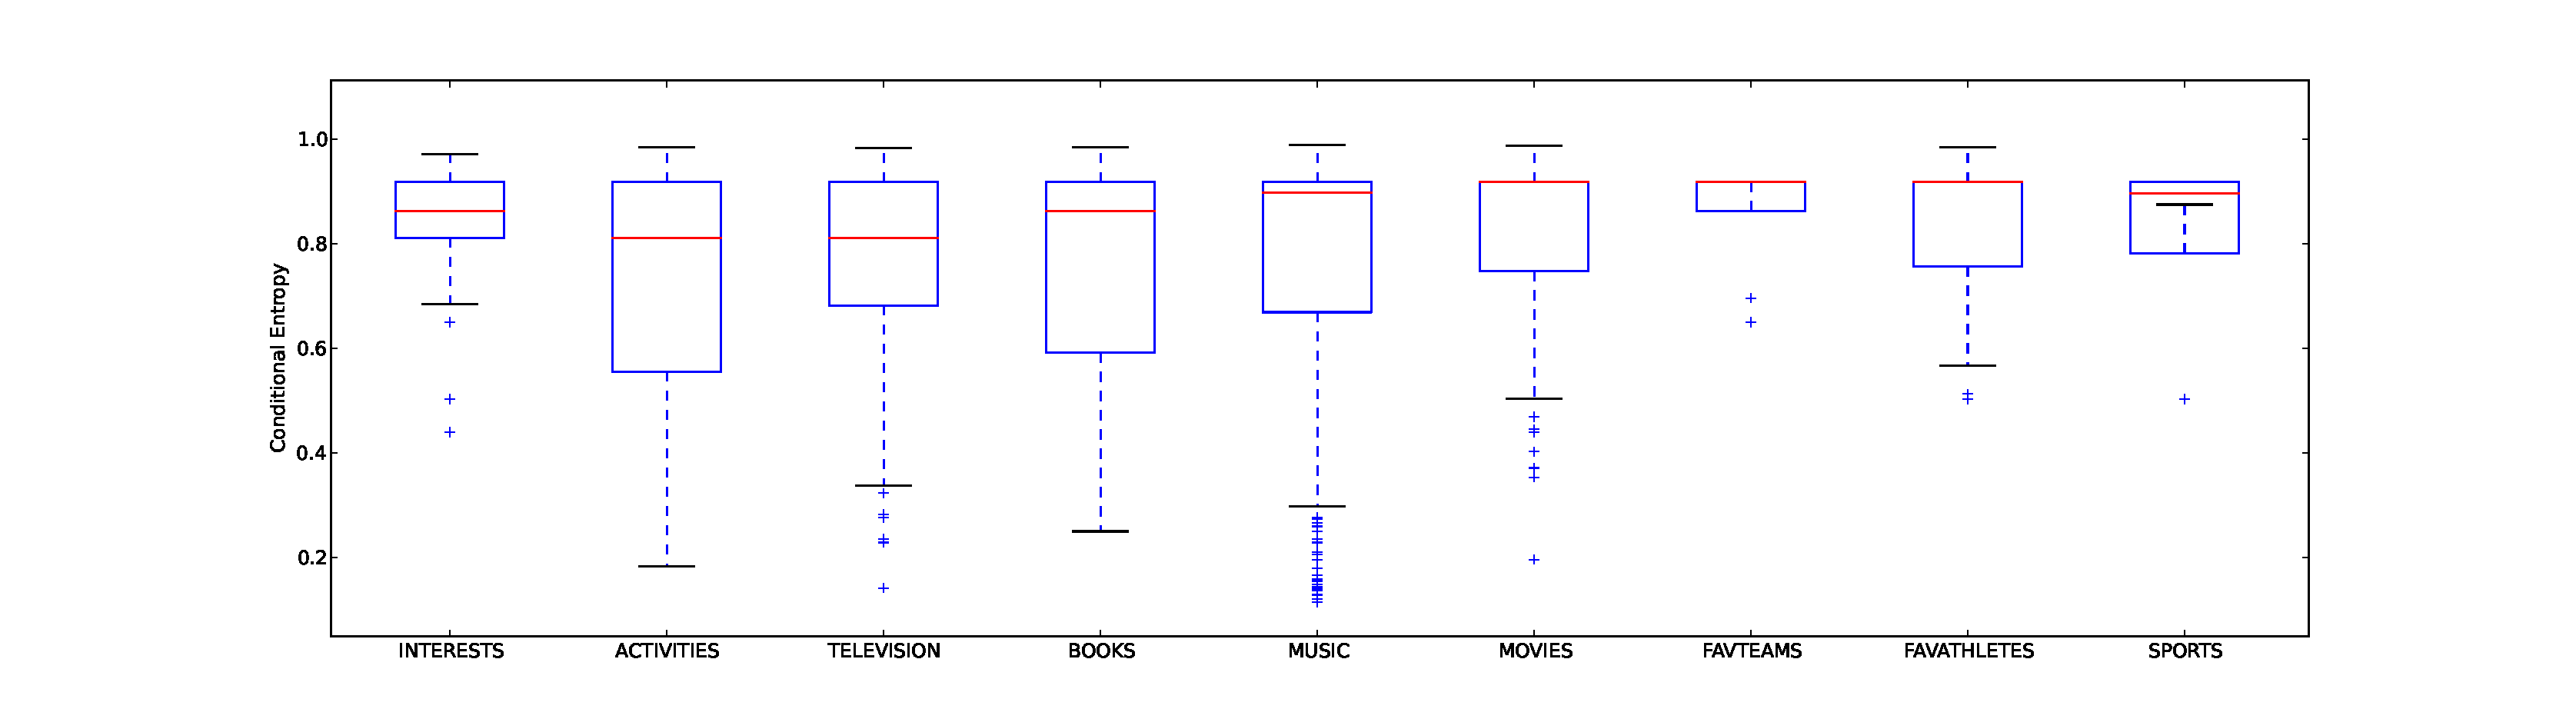
\includegraphics[width=180mm, height=35mm]{data/plots/boxPlots/CEvsFavTypes.eps}
\caption{Conditional entropy for top 1000 favourites breakdown by categories}
\label{Fig5}
\end{figure*}
%%%%%%%%%%%%%%%%%%%%%%%%%%%%%%%%%%%%%%%%%%%%%%%%%%%%%%%%%%%%%%%%%%%%%%%%%%%
